\subsection{PCA}
Prinsipalkomponentanalyse (PCA) er en veldig nyttig metode som benyttes til bl.a. mønstergjenkjenning, dimensjonalitetsreduksjon, klyngeanalyse, klassifisering og utliggerdeteksjon. Den baserer seg på noen viktige konsepter fra lineæralgebra.

\subsubsection{Matematisk bakgrunn}

La vektorene $\mathbf{x}, \mathbf{y} \in V$, der $V$ er et indreprouktrom. Disse vektorene er \textbf{ortogonale} dersom indreproduktet $\langle \mathbf{x}, \mathbf{y} \rangle = 0$. To underrom $A$ og $B$ er ortogonale dersom alle vektorer i $A$ er ortogonal med alle vektorer i $B$, og omvendt. En mengde vektorer $S$ er ortonormal dersom alle vektorene den inneholder er ortogonale med hverandre, og har norm 1.

\textbf{Projeksjonen} av vektoren $\mathbf{y}$ på $\mathbf{x}$ er gitt av

\begin{equation}
\textrm{Proj}_{\mathbf{x}} \mathbf{y} = \frac{\langle \mathbf{x}, \mathbf{y} \rangle}{|\mathbf{x}|^2}\mathbf{x}
	\label{eq_projection}
\end{equation}

En matrise $A$ kan sees på som en \textbf{lineærtransformasjon}, f.eks. en rotasjon eller en skalering i en viss retning.

\subsubsection{Tolkning av PCA}
PCA går kort oppsummert ut på å finne vektorer som best mulig forklarer varians i dataen, og som er ortogonale med hverandre. Håpet er at noen få av disse \textbf{prinsipale komponentene} forklarer en stor del av variansen. Metoden har en fin geometrisk tolkning. La $S$ være en sirkel, og $A$ være en lineærtransformasjon (f.eks. representert av en matrise). Da vil $A$ (med mindre den er singulær) ha egenvektorer $\mathbf{v}_1$ og $\mathbf{v}_2$. Disse vil da strekkes med faktorene $\sigma_i$, egenverdiene deres. Dette er vist i figur \ref{fig:pca_skvis}.

\begin{figure}[h]
	\centering
	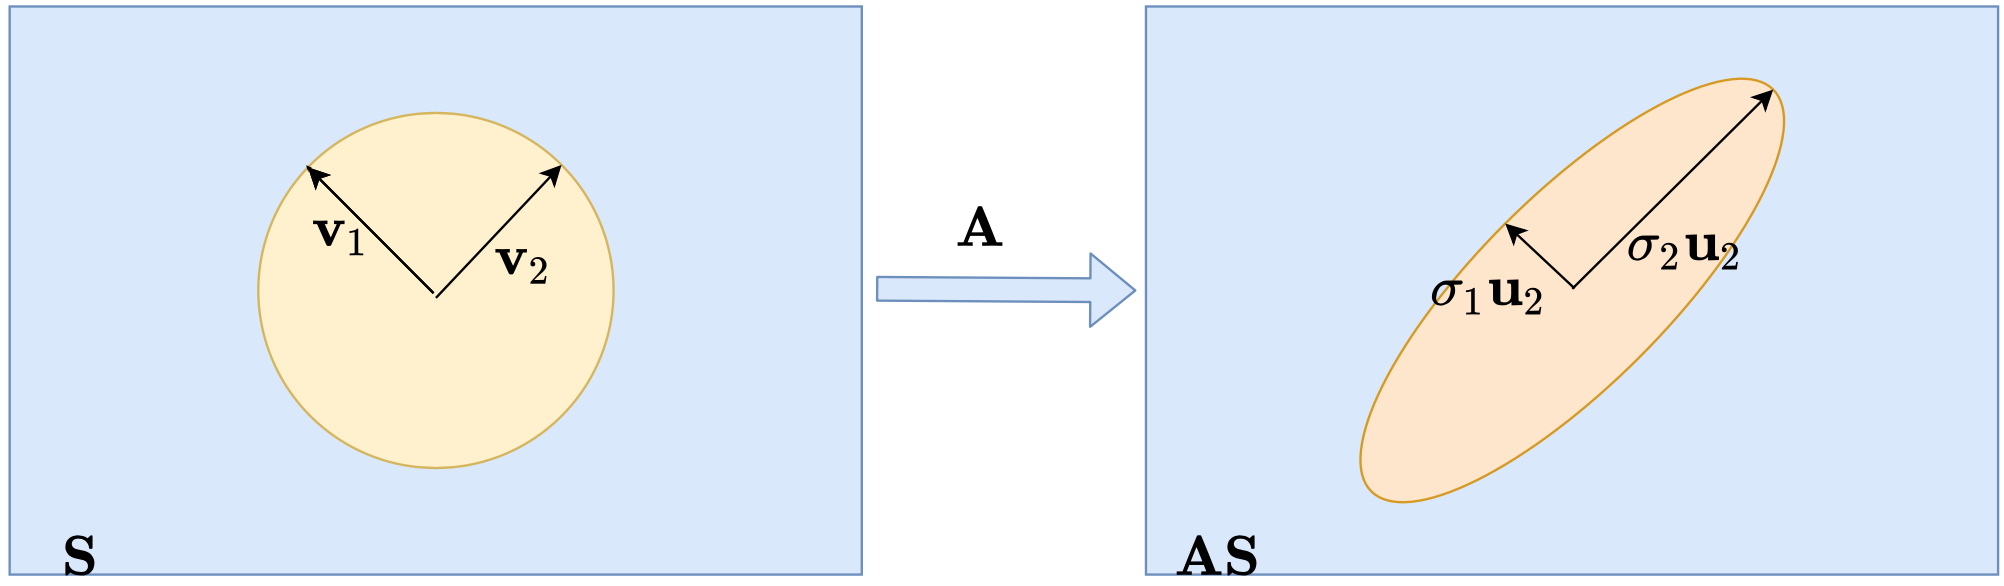
\includegraphics[width=\textwidth]{figurer/pca_skvis}
	\caption{Geometrisk tolkning av lineærtransformasjon}
	\label{fig:pca_skvis}
\end{figure}

For egenvektorer $\mathbf{v}_i$ med egenverdier $\sigma_i$ vil dermed

\begin{equation}
	A \mathbf{v}_j = \sigma_j \mathbf{u}_j
\end{equation}

For høyere dimensjon enn 2 (som i figuren) vil likningene være helt like. En hypersfære $\mathbf{V}$ av egenverdier transformeres av $A$ til en hyperellipse $\mathbf{U}$ under likningen

\begin{equation}
	A \mathbf{V} =\mathbf{U} \mathbf{\Sigma}
\end{equation}

Hvis egenvektorene til $A$ er lineært uavhengige, vil $\mathbf{V}$ være invertibel, og vi kan definere \textbf{singulærverdidekomposisjonen}

\begin{equation}
	A  =\mathbf{U} \mathbf{\Sigma} \mathbf{V}^*
\end{equation}

Ved å slå sammen matrisene $\mathbf{U} \mathbf{\Sigma}$ står vi igjen med en ny tolkning av $A$, forklart av kolonnene i $\mathbf{V}^*$ og kolonnene i $\mathbf{U} \mathbf{\Sigma}$. Dette er illustrert i figur \ref{fig:pca_komponentvis}. Mye av styrken til PCA ligger i at hvis $A$ har en lav nok underliggende dimensjon, kan vi approksimere $A$ ganske bra ved å kaste bort vektorene som svarer til lave singulærverdier $\sigma_i$. Modellordenen reduseres drastisk uten at vi mister viktig informasjon \Cooley.

\begin{figure}[h]
	\centering
	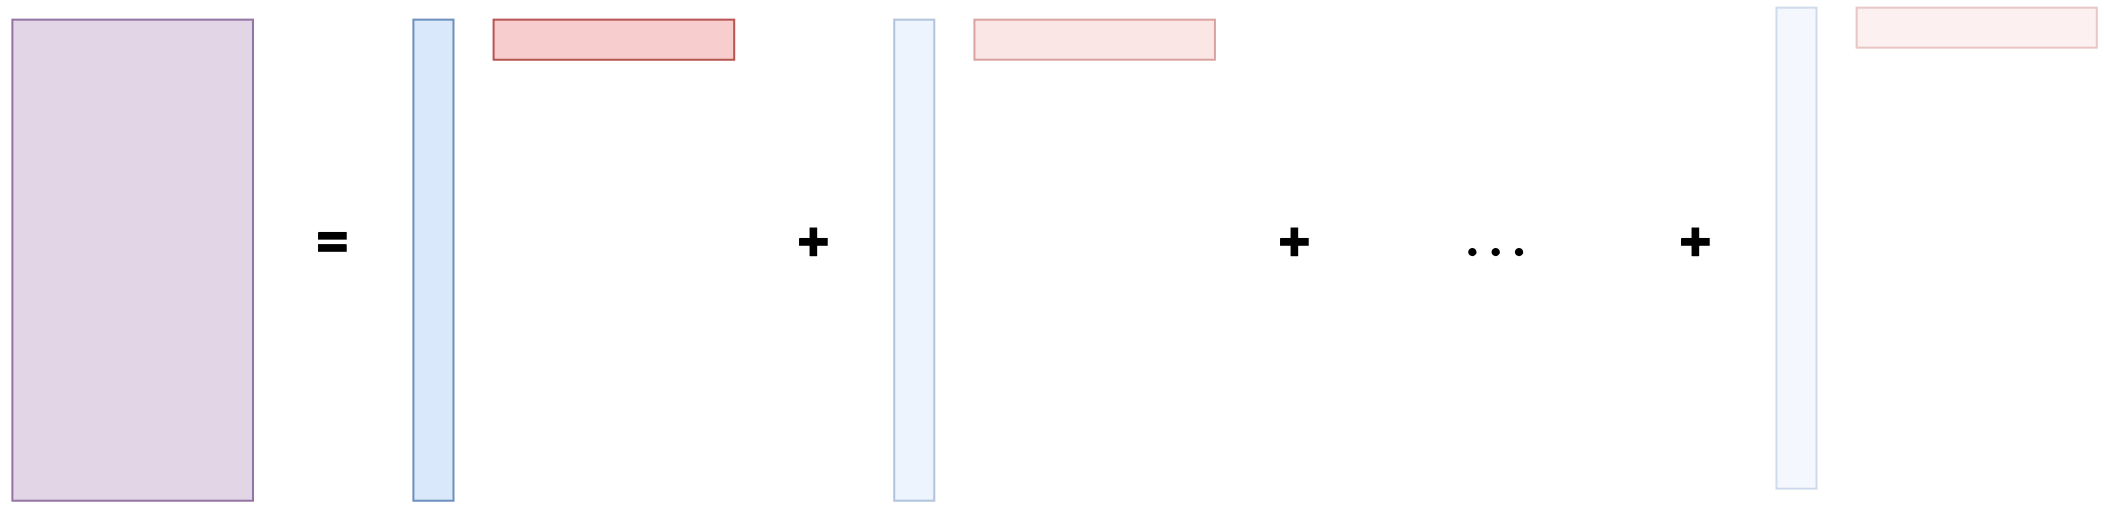
\includegraphics[width=\textwidth]{figurer/pca_komponentvis}
	\caption{Tolkning av SVD}
	\label{fig:pca_komponentvis}
\end{figure}

\subsubsection{Utledning av prinsipale komponenter}
Det finnes flere måter å finne de prinsipale komponentene. En av dem, kalt \textbf{egenverdidekomposisjonen}, baserer seg på at vi ønsker å maksimere variansen i ladningene $\mathbf{t} = \mathbf{Xp}$, der $X$ er dataen vår er $p$ er en prinsipal komponent (slik at $\mathbf{t}_j = \textrm{proj}_{\mathbf{p}} \mathbf{X}$, stol på dette). For å finne $p_1$, kan vi dermed løse optimeringsproblemet

\begin{equation}
	\max (\phi)=\boldsymbol{p}_{1}^{T} \boldsymbol{X}^{T} \boldsymbol{X} \boldsymbol{p}_{1}-\lambda\left(\boldsymbol{p}_{1}^{T} \boldsymbol{p}_{1}-1\right)
\end{equation}

som er funnet ved å inkludere begrensningen $\mathbf{p}_1^T \mathbf{p} = 1$ som Lagrange-multiplikator. Ved å derivere mhp. $\mathbf{p}_1$ og sette lik null, finner man at løsningen er gitt av likningen

\begin{equation}
	\mathbf{X}^T \mathbf{X} \mathbf{p}_1 = \lambda_1 \mathbf{p}_1
\end{equation}

Ved å innføre begrensningen $\mathbf{p}_1 \perp \mathbf{p}_2$ kan man finne at $\mathbf{p}_2$ kan finnes på akkurat tilsvarende vis osv. for de neste prinsipale komponentene.

PCA kan også gjøres ved å finne SVD-en til $X$, dette finnes det funksjoner for i de fleste \texttt{programmeringsspråk} som brukes til dataanalyse. Når man kjenner denne er dekomposisjonen av $\mathbf{X}$ i ladninger $\mathbf{p}_i$ med tilhørende score $\mathbf{t}_i$ gitt av

\begin{equation}
	\mathbf{X} = \mathbf{t}_1 \mathbf{p}_1^T + \mathbf{t}_2 \mathbf{p}_2^T + \cdots + \mathbf{E} = \sigma_1 \mathbf{u}_1 \mathbf{v}_1^T +  \sigma_2 \mathbf{u}_2 \mathbf{v}_2^T + \mathbf{E} 
\end{equation}


\subsubsection{NIPALS-algoritmen}
En effektiv metode for utregning av PC-er kalles Nonlinear Iterative Partial Least Squares (\textbf{NIPALS}). Denne ble blant annet brukt i tidlige versjoner av Google sin PageRank-algoritme. Algoritmen går ut på å iterativt finne hver prinsipale komponent, og å fjerne variabiliteten denne bidrar med før neste PC regnes ut. Noen fordeler med NIPALS er at man kan håndtere store datamengder i $\mathbf{X}$, at man kan håndtere manglende data, og at man er garantert konvergens. Pseudokoden under viser algoritmen. Merk at projeksjon av en matrise $X$ på en vektor $t$ etterfulgt av en normalisering mer kompakt kan skrives som 
\begin{equation}\frac{\textrm{proj}_t(X)}{|| \textrm{proj}_t(X) ||_2} = \frac{X^T t / t^T t}{|| X^T t / t^T t ||_2} = \frac{X^T t / t^T t}{\sqrt{(X^T t)^T (X^T t) / (t^T t)^2}} = \frac{X^T t}{|| X^T t ||_2}
\label{eq:normalisering_triks}
\end{equation}
Hovedideen bak NIPALS er å utlede ytreproduktene $t_i p_i^T$ én og én, med høyeste varians først. Disse vektorene finnes ved å iterativt tilpasse $p$ til $t$ vha. $X$, $t$ til $p$ vha. $X$, frem og tilbake helt til resultatet stabiliserer seg (dette kalles gjerne ``criss-cross regressions''). Pseudokode for NIPALS er som følger (merk at man antar at $X$ allerede er sentrert).

\begin{algorithm}
	\caption{NIPALS for PCA}\label{alg:nipals_pca} \begin{algorithmic}[1] \Procedure{NIPALS}{$X, n_\textrm{PCA}, t_\textrm{tol}$}\Comment{Numerisk utregning av PCA}
	\State $i \gets 1$
	\While{$i < n_\textrm{PCA}$}
	\State Initialisér $t_i$ (tilfeldig, eller som en av kolonnene i $X$)
	\While{Endring i $t_i > t_\textrm{tol}$}
	\State $p_i \gets \frac{X^T t_i}{|| X^T t_i ||_2}$ \Comment{Projeksjon av $X$ på $t_i$}
	\State $t_i \gets X p_i$ \Comment{Projeksjon av $X$ på $p_i$}
	\EndWhile
	\State $X \gets X - t_i p_i^T$ \Comment {Deflasjon}
	\State $i \gets i + 1$
	\EndWhile
\EndProcedure
\end{algorithmic}
\end{algorithm}

%\begin{algorithm}
%	\caption{NIPALS for PCA}
%	\label{alg:NIPALS_PCA}
%	\begin{algorithmic[1]}
%		\Procedure{NIPALS}{$X$}
%		\State Sentrér $X$-matrisen
%		\EndProcedure
%	\end{algorithmic}
%\end{algorithm}

\subsubsection{Visualisering av PCA}
Det finnes mange nyttige måter å bruke PCA på for å visualisere data. Kanskje blir dette kapitlet lengre etter hvert.

